% arara: pdflatex
% arara: biber
% arara: makeindex
% arara: nomencl
% arara: pdflatex
% arara: pdflatex

\documentclass[a4paper,12pt]{article}
%\RequirePackage[l2tabu,orthodox]{nag}

\usepackage{upreport}
\usepackage{tabularx}
\usepackage{amssymb}
\usepackage{siunitx}
\usepackage{gensymb}
\addbibresource{report.bib}
\title{Controllability Analysis of an Ethanol Water Distillation Column}
\subject{CBT }
\date{\today}

%Nomenclature unit command
\newcommand{\nomunit}[1]{%
\renewcommand{\nomentryend}{\hspace*{\fill}#1}}

% Create a custom user command or run the following 
%  makeindex %.nlo -s nomencl.ist -o %.nls
% execute this command after compiling your file once, then compile a second time to generate a nomenclature table



\begin{document}
\maketitle
\makecoverpage

\pagestyle{plain}
\thispagestyle{plain}
\pagenumbering{roman}

\begin{center}
\LARGE\textbf{\thetitle}
\end{center}

\section*{Synopsis}
\addcontentsline{toc}{section}{Synopysis}%
Welcome to the Noob's guide.
This section has only been included for reference on how to use it when comparing the source code to the resulting document.
Please continue to the Introduction, Section~\ref{sec:Introduction}.
\setcounter{page}{3}

\newpage
\tableofcontents

\iftotalfigures%
\newpage%
\listoffigures%
\fi

\iftotaltables%
\newpage%
\listoftables%
\fi

\newpage

%\chapter*{Nomenclature}
\printnomenclature
\newpage

\pagestyle{plain}
\setcounter{page}{1}
\pagenumbering{arabic}

\newpage

\section{Introduction}

Renewable energy is becoming a major role player in the world today. As people are starting to shift away from fossil fuel based technology and energy generation, the focus is shifting to alternative methods of energy (and fuel) production.

One such a method involves the use of ethanol as an alternative fuel. Ethanol particularly is an excellent contender for a major alternative fuel, as it can be produced from crops or by means of biological fermentation. [A lot of] research is currently done on methods to generate ethanol in order for it to power the future. 

Producing ethanol, however, is not the only problem to overcome. After the production process (usually from fermentation), the ethanol has to be separated from the product mixture in order to purify it. This poses to be a challenge (and a very energy intensive operation) due to the thermodynamic properties of the homogeneous mixture between water and ethanol. As noted in Figure~\ref{fig:vle-ethanol}, the system contains an azeotrope. This leads to very expensive separation operations, as pressure swing distillation has to be implemented for high purity separation.

\begin{figure}[tbph!]
	\centering
	\includegraphics[width=0.7\linewidth]{"Figures/VLE Ethanol 2"}
	\caption{Vapour Liquid Equilibrium (VLE) data for the water ethanol system at 1 bar.}
	\label{fig:vle-ethanol}
\end{figure}

In this report, an investigation regarding the controllability of the ethanol water separation process is investigated. The plant investigated is a pilot plant that is testing the feasibility for scale up of the process. Control has to implemented to ensure that the system reaches a steady state, as well as to improve the overall profitability by reducing the standard deviation in the product quality.

A plant wide control system will not be investigated. Only the distillation coloumn is analysed. The current proposed control system is discussed in Section~[REF!!!]. This report will investigate the validity of such a proposed control scheme, as well as the where the physical constrains in the system lies.
\newpage

\section{Process Model Description}

\subsection{System Diagram}

The Process Flow Diagram of the system, with all the relevant inputs, outputs and disturbances are displayed in Figure~\ref{fig:PFD}.

\begin{figure}[tbph]
	\centering
	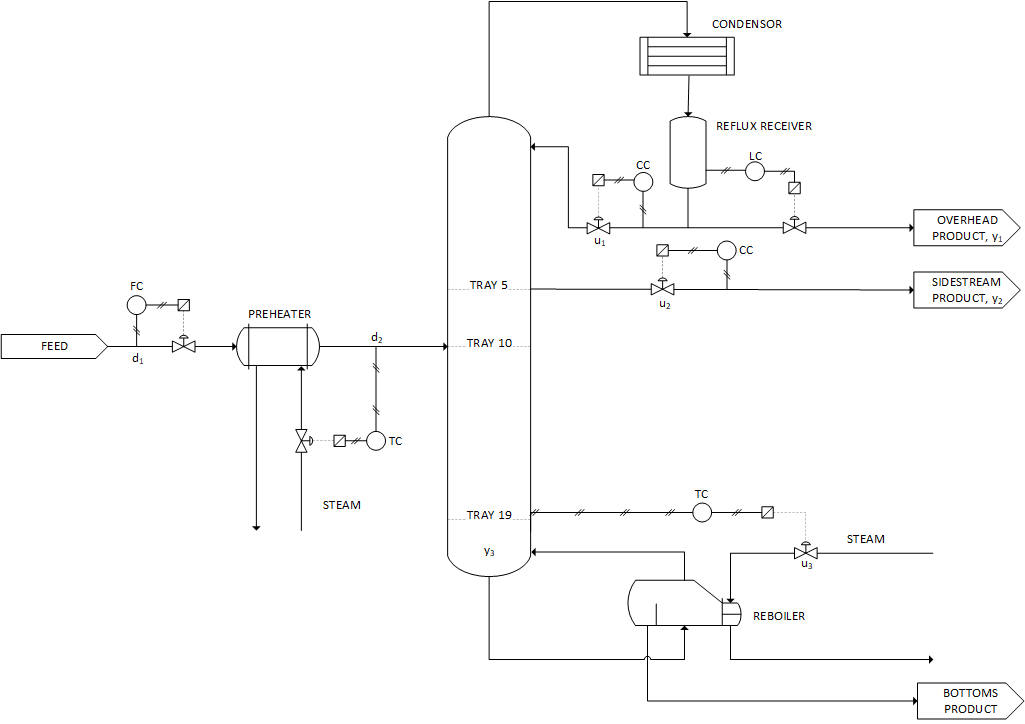
\includegraphics[width=0.9\linewidth]{Figures/Process_PFD}
	\caption{Process flow diagram of the system}
	\label{fig:PFD}
\end{figure}


\subsection{System Description}

The system involves the separation of water and ethanol (in a solution), with the aim of producing an ethanol product that can be used as an alternative fuel source.

The system can be summarized as follows:

\begin{itemize}
	\item The distillation column of the pilot scale plant is a 19 tray, 12 inch diameter column. 
	\item The column has variable feed and side stream draw off locations. 
	\item The side stream flow is varied to control the composition of the stream. 
	\item The distillate vapour draw off stream is fully condensed, and then separated into the reflux and product streams. 
	\item The product stream is set to control the level in the condenser, while the reflux stream controls the composition of the distillate product. 
	\item A kettle re-boiler is used to add energy to the column. Stream is the main utility. 
	\item The amount re-boiled bottoms product is controlled by varying the steam supplied to the re-boiler. 
	\item The feed temperature and flow rate can be controlled to simulate disturbances on the system. These variables are strictly defined as disturbances, as they are part of another section's (the bio-reactor or chemostat) control scheme.
	\item Currently all variables are controlled with single input single output (SISO) control loops.
	
\end{itemize}

\subsection{Measurement of Variables}

The compositions are measured/determined through various on-line sensors (densitrometry and refractometry). Temperatures are monitored using thermocouples. Flow rates are measured with thermal mass flow meters. Levels are measured by inference from static head, measured with a pressure sensor. The product model and serial numbers are not available.


\subsection{System Variables}

All variables in the ethanol water distillation coloumn system is summarised in Table~\ref{tab:Variables}. The current steady state values hold reference to the tested conditions on site.

\begin{table}[H]
	\centering
	\caption{Summary of all the model variables.}
	\begin{tabular}{cccc}
		\hline
		\multicolumn{4}{c}{Input Variables}                                       \\
		
		Variable & Description                       & Steady State Value & Units \\
		\hline
		$u_1$       & Reflux flow rate                  & 0.18               & gpm   \\
		$u_2$       & Side stream product flow rate     & 0.046              & gpm   \\
		$u_3$       & Reboiler steam pressure           & 20                 & psi   \\
		\hline
		\multicolumn{4}{c}{Output Variables}                                      \\
		
		Variable & Description                       & Steady State Value & Units \\
		\hline
		$y_1$       & Overhead ethanol mole fraction    & 0.7                & -     \\
		$y_2$       & Side stream ethanol mole fraction & 0.52               & -     \\
		$y_3$       & Tray \#19 temperature             & 92                 & \si{\celsius} \\
		\hline
		\multicolumn{4}{c}{Disturbance Variables}                                 \\
		
		Variable & Description                       & Steady State Value & Units \\
		\hline
		$d_1$       & Feed flow rate                    & 0.8                & gpm   \\
		$d_2$       & Feed temperature                  & 78                 & \si{\celsius} \\\hline
	\end{tabular}
	\label{tab:Variables}
\end{table}


\subsection{System Model}

The model was determined by conducting pulse testing on the system. In most cases a first order plus dead time model gave a sufficiently accurate fit to experimental data. The sum of squares of an adequate fit during model development was a values of greater than 0.98. In some relationships more complex dynamics had to be derived and a second order system with a first order lag and dead time, was used to accurately describe the impulse response (based on the same adequate fit method described above). The equations used for fitting were

\begin{equation}
	\frac{y_i(s)}{u_i(s)} = \frac{K_i e^{-\theta_is}}{\tau_i s + 1}
\end{equation}

for the first order plus dead time system, and 

\begin{equation}
	\frac{y_i(s)}{u_i(s)} = \frac{K_i (\tau_{1i}s + 1) e ^{-\theta_is +1}}{(\tau_{2i}s +1)(\tau_{3i}s +1)}
\end{equation}

for the relationships with more complex dynamics.

The fitting curves of two pulse tests are displayed in Figure~\ref{fig:test1} and Figure~\ref{fig:test2}. An important thing to note is that the unit of time is minutes, an therefore all responses and analysis will be conducted with this unit for time.

\begin{figure}[htbp]
	\centering
	\begin{minipage}{.48\textwidth}
		\centering
		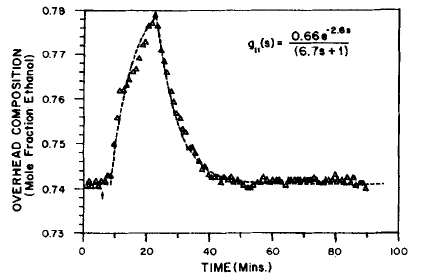
\includegraphics[width=\linewidth]{Figures/Pulse_test_1}
		\captionof{figure}{Overhead composition response to a pulse of 15 minutes duration in the reflux rate.}
		\label{fig:test1}
	\end{minipage}%
	\hfill
	\begin{minipage}{.48\textwidth}
		\centering
		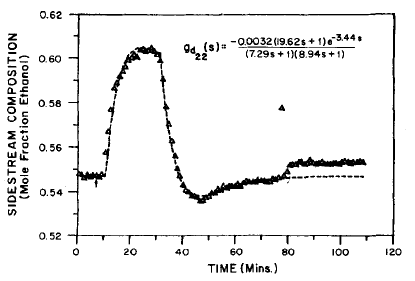
\includegraphics[width=\linewidth]{Figures/Pulse_test_2}
		\captionof{figure}{Side stream composition response to a pulse of 15 minutes duration in feed temperature.}
		\label{fig:test2}
	\end{minipage}
\end{figure}

The model was then written in the standard form of a linear MIMO system [REF!!!],

\begin{equation}
\textbf{y}(s) = \textbf{G}(s)\textbf{u}(s) + \textbf{G}_{d}(s)\textbf{d}(s)
\end{equation}

where

\begin{equation}
\hat{G}(s) = \begin{bmatrix}
G_{11} & G_{12} & G_{13} \\
G_{21} & G_{22} & G_{23} \\
G_{31} & G_{32} & G_{33} \\
\end{bmatrix} = \begin{bmatrix}
\frac{0.66e^{-2.6s}}{6.7s+1} & \frac{-0.61e^{-3.5s}}{8.64s+1} & \frac{-0.0049e^{-s}}{9.06s+1} \\
\frac{1.11e^{-6.5s}}{3.25s+1} & \frac{-2.36e^{-3s}}{5.0s+1} & \frac{-0.012e^{-1.2s}}{7.09s+1} \\
\frac{-34.68e^{-9.2s}}{8.15s+1} & \frac{46.2e^{-9.4s}}{10.9s+1} & \frac{0.87(11.61s+1)e^{-s}}{(3.89s+1)(18.8s+1)}
\end{bmatrix}
\end{equation}

and

\begin{equation}
\hat{G_d}(s) = \begin{bmatrix}
G_{d11} & G_{d12} \\
G_{d21} & G_{d22} \\
G_{d31} & G_{d32} \\
\end{bmatrix} = \begin{bmatrix}
\frac{0.14e^{-12s}}{6.2s+1} & \frac{-0.0011(26.32s+1)e^{-2.66s}}{(7.85s+1)(4.63s+1)} \\
\frac{0.53e^{-10.5s}}{6.9s+1} & \frac{-0.0032(19.62s+1)e^{-3.44s}}{(7.29s+1)(8.94s+1)} \\
\frac{-11.54e^{-0.6s}}{7.01s+1} & \frac{0.32e^{-2.6s}}{7.76s+1}
\end{bmatrix}
\end{equation}

\subsection{Scaling the System}

In order to perform a controllability analysis on the system, the system had to be scaled according to the method described in [Reff!!!].

In order to perform the scaling operation, the upper and lower limits of all the variables have to be defined. The initial boundary values of all system variables are summarized in Table~\ref{tab:Manipulated_variables_scaling}, Table~\ref{tab:Controlled_variables_scaling}, and Table~\ref{tab:Disturbance_variables_scaling}.

\begin{table}[H]
	\centering
	\caption{The boundaries of the manipulated variables in the system.}
	\begin{tabular}{cccc}
		\hline
		\textbf{\begin{tabular}[c]{@{}c@{}}Manipulated\\   Variable\end{tabular}} & \textbf{\begin{tabular}[c]{@{}c@{}}Lower \\ Constraint\end{tabular}} & \textbf{\begin{tabular}[c]{@{}c@{}}Upper \\ Constraint\end{tabular}} & \textbf{\begin{tabular}[c]{@{}c@{}}Steady State \\ Value\end{tabular}} \\\hline
		$u_1$, Reflux Flow Rate                                                      & 0.068                                                                & 0.245                                                                & 0.18                                                                   \\
		$u_2$, Side Stream Flow Rate                                                 & 0.00694                                                              & 0.1                                                                  & 0.046                                                                  \\
		$u_3$, Reboiler Steam Pressure                                               & 15.6                                                                 & 34                                                                   & 20                                                                                             
		\\\hline      
	\end{tabular}
	\label{tab:Manipulated_variables_scaling}
\end{table}

\begin{table}[H]
	\centering
	\caption{The boundaries of the controlled variables in the system.}
	\begin{tabular}{ccc}
		\hline
		\textbf{Controlled  Variable}         & \textbf{\begin{tabular}[c]{@{}c@{}}Maximum Set Point \\ Change\end{tabular}} & \textbf{Steady State Value} \\\hline
		$y_1$, Overhead Mole Fraction Ethanol    & 0.05                                                                         & 0.7                         \\
		$y_2$, Side Stream Mole Fraction Ethanol & 0.1                                                                          & 0.52                        \\
		$y_3$, Temperature on Tray \#19          & 8                                                                            & 92                         
		\\\hline      
	\end{tabular}
	\label{tab:Controlled_variables_scaling}
\end{table}

\begin{table}[H]
	\centering
	\caption{The boundaries of the controlled variables in the system.}
	\begin{tabular}{cccc}
		\hline
		\textbf{\begin{tabular}[c]{@{}c@{}}Disturbance\\   Variable\end{tabular}} & \textbf{\begin{tabular}[c]{@{}c@{}}Lower \\ Constraint\end{tabular}} & \textbf{\begin{tabular}[c]{@{}c@{}}Upper \\ Constraint\end{tabular}} & \textbf{\begin{tabular}[c]{@{}c@{}}Steady State \\ Value\end{tabular}} \\\hline
		d1, Feed Flow Rate            & 0.6                       & 1.1                       & 0.8                         \\
		d2, Feed Temperature          & 50                        & 102                       & 78                         
		\\\hline      
	\end{tabular}
	\label{tab:Disturbance_variables_scaling}
\end{table}

Using the information above the following matrices can be deduced, that will be used to scale the system

\begin{equation}
	D_e = \begin{bmatrix}
	0.01 & 0 & 0 \\
	0 & 0.01 & 0 \\
	0 & 0 & 4 \\
	\end{bmatrix}
\end{equation}

\begin{equation}
D_u = \begin{bmatrix}
0.065 & 0 & 0 \\
0 & 0.03906 & 0 \\
0 & 0 & 4.4 \\
\end{bmatrix}
\end{equation}

\begin{equation}
D_d = \begin{bmatrix}
0.3 & 0 \\
0 & 28 \\
\end{bmatrix}
\end{equation}

\begin{equation}
r = \begin{bmatrix}
0.05 & 0 & 0 \\
0 & 0.1 & 0 \\
0 & 0 & 8 \\
\end{bmatrix}
\end{equation}

Using the above matrices, the scaled system can be calculated using the following equations from [REF!!!],

\begin{equation}
	\label{eq: Scaling 1}
	G = D_e ^{-1}\hat{G}D_u
\end{equation}

\begin{equation}
	\label{eq: Scaling 2}
	G_d = D_e ^{-1}\hat{G_d}D_d
\end{equation}

From Equation~\ref{eq: Scaling 1} and Equation~\ref{eq: Scaling 2}, the scaled system can be written as 

\begin{equation}
G(s) = \begin{bmatrix}
G_{11} & G_{12} & G_{13} \\
G_{21} & G_{22} & G_{23} \\
G_{31} & G_{32} & G_{33} \\
\end{bmatrix} = \begin{bmatrix}
\frac{4.29e^{-2.6s}}{6.7s+1} & \frac{-2.38266e^{-3.5s}}{8.64s+1} & \frac{-2.156e^{-s}}{9.06s+1} \\
\frac{7.215e^{-6.5s}}{3.25s+1} & \frac{-9.21816e^{-3s}}{5.0s+1} & \frac{-2.156e^{-1.2s}}{7.09s+1} \\
\frac{-0.56355e^{-9.2s}}{8.15s+1} & \frac{0.451143e^{-9.4s}}{10.9s+1} & \frac{1.1(10.1007s+0.87)e^{-s}}{(3.89s+1)(18.8s+1)}
\end{bmatrix}
\end{equation}

and

\begin{equation}
G_d(s) = \begin{bmatrix}
G_{d11} & G_{d12} \\
G_{d21} & G_{d22} \\
G_{d31} & G_{d32} \\
\end{bmatrix} = \begin{bmatrix}
\frac{4.2e^{-12s}}{6.2s+1} & \frac{-2800(0.028952s+0.0011)e^{-2.66s}}{(7.85s+1)(4.63s+1)} \\
\frac{15.9e^{-10.5s}}{6.9s+1} & \frac{-2800(-0.062784s+0.0032)e^{-3.44s}}{(7.29s+1)(8.94s+1)} \\
\frac{-0.8655e^{-0.6s}}{7.01s+1} & \frac{2.24e^{-2.6s}}{7.76s+1}
\end{bmatrix}
\end{equation}

with 

\begin{equation}
R = \begin{bmatrix}
5 & 0 & 0 \\
0 & 10 & 0 \\
0 & 0 & 2 \\
\end{bmatrix}
\end{equation}
\newpage

\section{Controllability Analysis}

A full controllability analysis was performed on the system to establish whether:

\begin{enumerate}
	\item The system has acceptable set point tracking characteristics.
	\item The system has acceptable disturbance rejection characteristics.
\end{enumerate}

The method used is described in \textcite{skogestad}. 

\subsection{Minimal Realisation of the System}

The system written in the transfer function notation is in no danger of not being a minimal realizable system. It is only when the system is converted to state space notation it runs the risk of not being a minimal realization. 

When converting the transfer function model to a state space realisation of the system, it has to be noted that all dead time that is inherent to the system is ignored, as state space realizations cannot deal with dead time. The system was however converted to its state space realization, in order to cross check the calculated poles and zeros of the system.

The minimum state space realization of the system is given below.

\subsection{Functional Controllability}

The system has to be checked for functional controllability. This implies that outputs should be able to be controlled independently. There are two factors that have to be considered when checking for functional controllability of a system, namely

\begin{enumerate}
	\item There have to be at least as many inputs as there are outputs
	\item The rank of $G(s)$ should be greater than the number of outputs.
\end{enumerate} 

For consideration 1, mentioned above, the number of inputs and outputs in the system is equal. This criteria is therefore satisfied by the system.

For consideration 2, the minimum singular value (or $\underline{\sigma}$) of $G(j\omega)$ should be non-zero. In order to determine whether the system satisfies this criteria, all the singular values, of all the outputs were computed of a wide frequency range. A bode diagram displaying the result can be seem in Figure~\ref{fig:gs-singular-values}.

\begin{figure}
	\centering
	\includegraphics[width=0.7\linewidth]{"Figures/G(s) Singular Values"}
	\caption{The singular values of $G(j\omega)$.}
	\label{fig:gs-singular-values}
\end{figure}

As is clear from Figure~\ref{fig:gs-singular-values}, $\underline{\omega}$ never reaches zero, although it does approach zero as the frequency goes to infinity. 

Based on the above information, it can be concluded that the system is indeed functionally controllable. This implies that the system's rank is equal to the amount of outputs that the system has.

The current selected inputs and outputs can therefore be controlled with adequate independence. This further implies that outputs can return a response by some combination of the input variables.

A system that is functionally uncontrollable will have output responses remaining zero, whenever any combination of an input step function is applied to the system. This therefore results in an output that can in no way be controlled by the inputs, as the inputs do not effect the outputs at all.

\subsection{System Poles}
\label{sec:System Poles}
\subsubsection{Calculating the System Poles}

The poles of the system was calculated. The system has a total  number of 25 poles. Some of the poles calculated are listed in Table~\ref{tab: Poles of system}. These only contain the more interesting poles. Please refer to Figure~\ref{fig:polesandzeros} for the locations of all the calculated poles.

\begin{table}[H]
	\centering
	\caption{The poles of the system.}
	\begin{tabular}{ccc}
		\hline
		\textbf{Pole} & \textbf{Real Part} & \textbf{Imaginary Part} \\\hline
		$p_1$            & -0.31            & 0                       \\
		$p_2$            & -0.26            & 0                       \\
		$p_3$            & -0.20            & 0                 \\
		$p_4$            & -0.23            & 0                 \\
		$p_5$            & 0.036             & 0.23                  \\
		$p_6$            & 0.036             & -0.23   \\\hline             
	\end{tabular}
	\label{tab: Poles of system}
\end{table}

\subsubsection{Calculating the System Pole Directions}
\label{sec:Pole Directions}

The pole directions of the system was calculated by substituting the relevant pole values into $G(s)$ and calculating the input and output directions poles. This was only done for the poles occurring in the Right Hand Plane (RHP). The calculated pole directions are listed in Table~\ref{tab: Pole Directions of system}.

\begin{table}[H]
	\centering
	\caption{The pole directions of the system.}
	\begin{tabular}{ccc}
		\hline
		\textbf{Pole} & \textbf{Input Direction ($V$)} & \textbf{Output Direction ($U$)} \\\hline
		$p_5$            & $ \begin{bmatrix} -0.71 \\ 0.68 + 0.12j \\ 0.13 + 0.05j\end{bmatrix} $ & $ \begin{bmatrix} -0.19+0.22j \\ -0.79+0.53j \\ 0.02 -0.03j\end{bmatrix} $ \\
		$p_6$            & $ \begin{bmatrix} -0.71 \\ 0.68 - 0.12j \\ 0.13 -0.05j\end{bmatrix} $ & $ \begin{bmatrix} -0.19-0.22j \\ -0.79+0.53j \\ 0.02 - 0.03j\end{bmatrix} $ \\\hline             
	\end{tabular}
	\label{tab: Pole Directions of system}
\end{table}

\begin{table}[H]
	\centering
	\caption{The pole directions of the system in phasor notation.}
	\begin{tabular}{ccc}
		\hline
		\textbf{Pole} & \textbf{Input Direction ($V$)} & \textbf{Output Direction ($U$)} \\\hline
		$p_5$            & $ \begin{bmatrix} 0.71 \\ 0.69\angle10.1^{\circ} \\ 0.13\angle19.6^{\circ}\end{bmatrix} $ & $ \begin{bmatrix} 0.29\angle130.9^{\circ} \\ 0.96\angle146.0^{\circ} \\ 0.04\angle-48.9^{\circ}\end{bmatrix} $ \\
		$p_6$            & $ \begin{bmatrix} 0.71 \\ 0.69\angle-10.1^{\circ} \\ 0.13\angle-19.6^{\circ}\end{bmatrix} $ & $ \begin{bmatrix} 0.29\angle-130.9^{\circ} \\ 0.96\angle-146.0^{\circ} \\ 0.04\angle48.9^{\circ}\end{bmatrix} $ \\\hline             
	\end{tabular}
	\label{tab: Pole Directions of system Phasor Notation}
\end{table}


\subsubsection{Discussion of System Poles}

Most of the calculated system poles are in the open left hand plane (LHP). There is however one pair of complex poles that lie in the open RHP. These poles will cause instability when they are approached. To gain better understanding into the what causes the system to behave in this way, the pole directions were calculated in Section~\ref{sec:Pole Directions}. 

Using Table~\ref{tab: Pole Directions of system Phasor Notation} as reference the directions of the system in this unstable condition can be analysed. From the table it is clear that the unstable response exists whenever the variable $y_2$ (side stream composition) is increased by almost one unit. This cannot be done without effecting the output $y_1$, as it is increase by almost a third of a unit during this response. Only the temperature can remain relatively unaffected during the response. We also note that $y_1$ and $y_2$ are in phase with one another, while$y_3$ is out of phase the first two outputs.

Looking at the input directions in Table~\ref{tab: Pole Directions of system Phasor Notation}, it is clear that the described output is obtained from manipulation of $u_1$ and $u_2$. While $u_3$ is manipulated slightly, its amplitude is well below the amplitude of the other system inputs. We can therefore generalize and say that the pole exists when reflux flow rate is increased and side stream draw off flow rate is decreased by the same amount. One small thing to note, is that the input $u_1$ does not have a phasor notation, as it is not a complex variable.

From the above it is clear, that the side stream composition cannot stepped one unit by manipulating the side stream flow rate and reflux flow rate exclusively. This composition will have to be controlled other combinations of measured variable, for the system to remain stable.

From a production point of view, this will not likely pose to be problem, as it is not a scenario that is very likely to exist. As mentioned earlier, the main ethanol product is in the distillate of the column. The shift described by this pole, will decrease both the distillate and side stream flow rates, resulting in a plummeting production profit as the product streams are redirected to waste or downstream processing (the bottoms flow).
 

\subsection{System Zeros}
\label{sec:System Zeros}
\subsubsection{Calculating the System Zeros}

The system zeros were calculated. The system contains a total number of nine zeros, all of them located in the left hand plane (LHP). The system zeros are given in Table~\ref{tab: Zeros of system}.

\begin{table}[H]
	\centering
	\caption{The zeros of the system.}
	\begin{tabular}{ccc}
		\hline
		\textbf{Zero} & \textbf{Real Part} & \textbf{Imaginary Part} \\\hline
		$z_1$            & -0.3077            & 0                       \\
		$z_2$            & -0.2571            & 0                       \\
		$z_3$            & -0.2            & 0                  \\
		$z_4$            & -0.1493            & 0                 \\
		$z_5$            & -0.1227             & 0                  \\
		$z_6$            & -0.1157             & 0   \\
		$z_7$            & -0.1104             & 0   \\
		$z_8$            & -0.0917             & 0   \\
		$z_9$            & -0.0532             & 0   \\\hline             
	\end{tabular}
	\label{tab: Zeros of system}
\end{table}

Since all zeros are in the LHP, and will in no way cause limitations on the bandwidth or stability of the system, the directions of the zeros were not calculated.

\subsubsection{Discussion of System Zeros}

The system zeros exists for values of $s$ where the system $G(s)$ loses rank. The zeros calculated, are transmission zeros of the system as they do not relate to the zeros of the elements that make up the transfer function matrix $G(s)$. It is clear that there are no RHP zeros, and no further analysis of the zeros are required, as there are no limitations imposed by Left Hand Plane (LHP) zeros. 

LHP zeros will mostly cause high overshoots during control, but this does not pose as a stability concern for the system and will in no way limit the bandwidth of the system.

\begin{figure}[H]
	\centering
	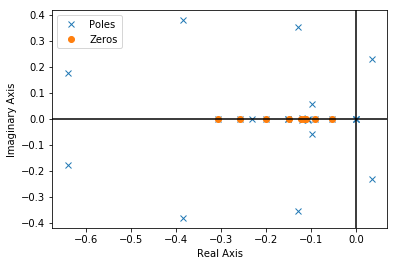
\includegraphics[width=0.7\linewidth]{Figures/Poles_and_Zeros}
	\caption{A graphical representation of the system's poles and zeros.}
	\label{fig:polesandzeros}
\end{figure}

\subsection{RGA Values of the System}
\label{sec:RGA Calculation}

The Routh Gain Array (RGA) of $G(j\omega)$ was calculated, for all values of $\omega$, where the frequency domain analysis held stable. This enables the analysis of RGA values not only for at the crossover frequencies, but at all other frequencies to thoroughly check for large RGA elements that will render a plant that is difficult to control. Due to dead time in the system, the frequency response of the RGA calculation tends to become severely unstable at higher frequencies. Luckily, spikes in the response will always tend to go downward, and the maximum RGA values can still be calculated. The calculated RGA analysis can be seen in Figure~\ref{fig:rga-values}.

\begin{figure}[H]
	\centering
	\includegraphics[width=0.7\linewidth]{"Figures/RGA Values"}
	\caption{The diagonal values of RGA matrix, $\Lambda$, over a wide range of frequencies.}
	\label{fig:rga-values}
\end{figure}

To verify that the off-diagonal values remain within acceptable ranges, the RGA of $G(0)$ and $G(j\omega)$ with $\omega = 10^{-1}$ was calculated. The two matrices calculated are

\begin{equation}
	\Lambda G(0) = \begin{bmatrix}
	2.11 & -0.84 & -0.26\\
	-0.59 & 1.67 & -0.08\\
	-0.52 & 0.17 & 1.34
	\end{bmatrix}
\end{equation}

\begin{equation}
\Lambda G(j10^{-1}) = \begin{bmatrix}
1.36 & -0.33 & -0.03\\
-0.37 & 1.34 & -0.03\\
0.02 & -0.02 & 1.00
\end{bmatrix}
\end{equation}

\subsection{Singular Values of the System}

The minimum singular value is a useful tool when doing controllability an analysis. The minimum singular value for this system is depicted in Figure~\ref{fig:gs-singular-values}.

The minimum singular value should be as large as possible, especially at frequencies where control is needed \parencite{skogestad}.

From Figure`\ref{fig:gs-singular-values}, it is clear that

\begin{equation}
	\label{eq: Min singular alue criteria}
	\underline{\sigma}(G(j\omega)) < 1 , \forall \omega
\end{equation}

This implies that it is not possible to make output changes of unit magnitude, by using inputs of unit magnitude for any values of $\omega$. 

This is bad from a controllability point of view, especially when considering set-point tracking. When tracking set-points, outputs ideally have to controlled by making single set-point changes. This enables the use of a decentralized controller. An example of such a controller (represented in a standard transfer function notation) is

\begin{equation}
	K(s) = \begin{bmatrix}
	\frac{K_1}{\tau_1s + 1} & 0 & 0\\
	 0 &\frac{K_2}{\tau_2s + 1} & 0\\
	 0 & 0 & \frac{K_3}{\tau_3s + 1}\\
	\end{bmatrix}
\end{equation} 

With the current plant configuration and design, the use of a decentralized controller is possible, but adequate set-point tracking will not be possible as the outputs will not reach the set-points on the high and/or low set-point values.

For example; when the temperature on tray \# 19 , $y_3$, is controlled between 88 and 96 $^{\circ}$, set-point tracking by manipulation of the stream feed pressure, $u_3$, will be acceptable (when considering a decentralized controller that contains an integral component). Acceptable set-point tracking includes: fast response time, elimination of error, robust responses. An adequately fast response time for this system will be around 45 minutes. With a high enough gain value, $K_{c3}$, this will be achieved. The integral component of the controller will eliminate the error completely over time, given that the integral component of the controller, $\tau_{c3}$, is large enough. Robust control will be achieved by tuning the controller values after initial implementation.

Now, when considering set-points on the outer limits of the control range for $y_3$, the control system will not perform acceptably. For instance when the set-point of $y_3$ is set to ranges 84 to 88 $\celsius$ or 96 to 100 $\celsius$, the response time of the set-point change may still be good, but the error will not be able to be cancelled. This is due to the minimum singular value of the system being smaller than 1. The unit change in the input, $u_3$, will not cause a unit change in the output, $y_3$. Since the system is scaled, this simply means that the outer set-points cannot be reached by only manipulating one input variable. 

The situation discussed above, only applies to the $y_3$ and $u_3$ control pairing. From Figure~\ref{fig:gs-singular-values}, it is clear that the criteria stated in Equation~\ref{eq: Min singular alue criteria} is satisfied for the $y_2$ and $u_2$ paring for all frequencies where $\omega<0.28$. Similarly, the criteria in Equation~\ref{eq: Min singular alue criteria} is satisfied in the $y_1$ and $u_1$ pairing for all frequencies where $\omega < 2.97$.

The are a few options for improvement and successful implementation of the control system. They are

\begin{enumerate}
	\item To implement a controller that is not decentralised. This controller can still control $y_1$ an $y_2$ using $u_1$ and $u_2$. $y_3$ will then be controlled by a combination of $u_3$ and $u_2$ (this follows from the RGA matrix analysis, where $u_1$ is negative with regard to $y_3$). The controller equation will then take the form of
	\begin{equation}
		K(s) = \begin{bmatrix}
		\frac{K_1}{\tau_1s + 1} & 0 & 0\\
		0 &\frac{K_2}{\tau_2s + 1} & 0\\
		0 & \frac{K_{3_1}}{\tau_{3_1}s + 1} & \frac{K_{3_2}}{\tau_{3_2}s + 1}\\
		\end{bmatrix}
	\end{equation}
	
	While this will ensure that acceptable set-point tracking of the bottom tray temperature is accomplished, there will be a loss in the performance and robustness of the control in the side-stream composition.
	
	\item Increase the size of the control valves controlling the stream pressure. This will increase the overall gain in the system, shifting the singular values in an upward direction. This will render acceptable set-point tracking of all parameters.
	
	\item Lower the required range wherein set-point tracking has to be performed. 
\end{enumerate}

\subsection{System Bandwidth}

The bandwidth of the system is the maximum frequency where sensible control can still be implemented. Mathematically it is where the sensitivity function of the system first crosses $1/\sqrt{2}$, or

\begin{equation}
	|S(j\omega)| = \frac{1}{\sqrt{2}}
\end{equation}

Since no controller is implemented as yet, there is no way of calculating the sensitivity function. As discussed in Section~\ref{sec:System Poles} and Section~\ref{sec:System Zeros}, there are no Right Hand Plane (RHP) zeros in this system. There are two RHP poles present, that will impose limitation on the on the system. The limitation imposed on the system are

\begin{enumerate}
	\item Limitations on the input usage. This constrains the amount of gain that can be applied to the system with a controller. In general
	
	\begin{equation}
		||KS||_{\infty} \geq ||u^H_p G_s(p)^{-1}||_2
	\end{equation}
	This is not entirely relevant to this report, as it entails the implementation of a controller. While this upper bound may be useful to assist with the design of the controller, the main focus of this report will remain on the controllability of the system.
	
	\item Limitations on the bandwidth. In short, the system has to react fast enough to avoid running into stability problems. The RHP pole therefore gives a minimum bound on the bandwidth (unlike RHP-zeros, which impose maximum bound constraints). According to \textcite{skogestad} the minimum closed loop bandwidth is 
	
	\begin{equation}
		\omega_B \geq 2|p|
	\end{equation}
	
	Using the equation the minimum bandwidth can be calculate to be $\omega_B = 0.46$. This gives a response time of less than 2.15 minutes.
\end{enumerate}

The system also contains a lot of dead time. There is dead time in each transfer function, as this is it is inherent to the fitting function used to build the model. There are constraints on the bandwidth due to this dead time. To visualize the dead time inherent to the system, please refer to Equation~\ref{eq:Deadtime Matrix}. This equation, simply named the dead time matrix, is a representation of the dead time elements ($\theta_{ij}$) for the respective transfer functions.

\begin{equation}
	\label{eq:Deadtime Matrix}
	\Theta = \begin{bmatrix}
	 2.6 & 6.5 & 9.2 \\
	 3.5 & 3.0 & 9.4 \\
	 1.0 & 1.2 & 1.0\\
	\end{bmatrix}
\end{equation} 

The lower bound time delay for each output (or contained within each row of $\Theta$) is of interest. This is because the minimum time for any input to effect the relevant output ($\theta_i^{min}$), can be seen as the delay that is pinned to output $y_i$. Alternatively this statement can be represented mathematically as 

\begin{equation}
	\theta_i^{min} = \min_j \theta_{ij}
\end{equation}

The bandwidth of input $u_i$ is then limited by the lower bound $1/\theta_i$. Table~\ref{tab:Bandwidths}, contains a summary of the bandwidth limitations of the system.

\begin{table}[H]
	\centering
	\begin{tabular}{ccc}
		\hline
		\textbf{Input} & \textbf{Theta} & \textbf{Bandwidth} \\
		\hline
		$y_1$             & 2.6            & 0.38               \\
		$y_2$             & 3.0              & 0.33               \\
		$y_3$             & 1.0              & 1.0                 \\\hline
	\end{tabular}
	\caption{Bandwidth limitations imposed by time delays.}
	\label{tab:Bandwidths}
\end{table}

While these limitations are in no way ideal, they do not pose to be a major threat for the control of the system. There are a few conclusions that can be drawn from this, namely

\begin{enumerate}
	\item When looking at Equation~\ref{eq:Deadtime Matrix} together with Section~\ref{sec:RGA Calculation}, it is clear that the diagonal elements that are paired in the RGA matrix, also contain the least amount of dead time. This is good, as it is obvious that you want to control a variable with an input that does not take long to effect the variable. Pairing of the variables are therefore made relatively straight forward.
	\item The delays imposed are not that significant when considering the desired response times for the control system. Required response times for the variables of the distillation column range between 30 and 60 minutes. The maximum delay calculated here (3 minutes), is relatively small and a low gain controller should be able to control the system with adequate performance. The performance of the system is discussed in more detail later in the report.
	\item Controlled variables $y_1$ and $y_2$ are more constrained by the RHP pole that exist than the delay that is inherent to these variables. Only $y_3$ is limited by the delay of the response.
\end{enumerate}

\subsection{Disturbance Rejection}

In order for the system to successfully reject disturbances, tight control and large bandwidths are required to when disturbances are large or "fast". 

To evaluate a MIMO system's ability to reject disturbances, the disturbance directions have to be evaluated (which is not the case when considering a SISO system). 

The model contains two disturbances, each having it's own associated direction. The disturbance directions are defined as

\begin{equation}
	y_d = \frac{1}{||g_d||_2}g_d
\end{equation}

where $g_d$ represents the effect of a single disturbance on the outputs ($y = g_dd$).

The disturbance directions for both disturbances were evaluated for all frequencies. The results can be seem in Figure~\ref{fig:disturbance-direction}.

\begin{figure}[H]
	\centering
	\includegraphics[width=0.7\linewidth]{"Figures/Disturbance Direction"}
	\caption{The disturbance directions as a function of frequency.}
	\label{fig:disturbance-direction}
\end{figure}

Now, following that the system has been scaled (Section~\ref{sec:Scaling}), we can say that the worst-case disturbance to be selected is $|d_i(\omega)| = 1$. Using this, and the fact that with feedback control we have $e = Sg_dd$, the disturbance performance objectives are then satisfied when

\begin{equation}
	||Sg_d||_{\infty} < 1
\end{equation}

Note that $S(s)$ could not actually be calculated. This is because no controller has yet been designed for the system. To gain better understanding of the disturbances in the system, a proportional decentralized controller with a gain of 1 (for all elemnts) was used.

\textcite{skogestad} used the above and derived tight bounds on the sensitivity function and loop gain for MIMO syste, considering the disturbance directions as well. For the system to adequately reject disturbances, we at least require that 

\begin{equation}
	\label{eq: Disturbance Criteria 1}
	\underline{\sigma}(S) < \frac{1}{||g_d||_2}
\end{equation}

Where $S$ is the sensitivity function of the transfer function model, or can be given mathematically as 

\begin{equation}
	S = (I + G)^{-1}
\end{equation}

for a negative feedback loop.

Equation~\ref{eq: Disturbance Criteria 1} can be represented graphically. The left-hand side and right-hand side of the equation was plotted for all values of $\omega$. The results are displayed in Figure~\ref{fig:disturbance-analysis-1}.

\begin{figure}[H]
	\centering
	\includegraphics[width=0.7\linewidth]{"Figures/Disturbance Analysis 1"}
	\caption{The disturbance directions with respect to the singular values of the sensitivity of $G(s)$, $S(s)$.}
	\label{fig:disturbance-analysis-1}
\end{figure}

From Figure~\ref{fig:disturbance-analysis-1}, it is clear that, based on the criteria stated in Equation~\ref{eq: Disturbance Criteria 1}, there may be some problems regarding disturbance rejection (especially at low frequencies). To share more light on the causes of the problem, an more in depth analysis is conducted below.

\subsection{Disturbances and Input Saturation}

\subsubsection{Analysis for Perfect Control}
Here it is asked whether disturbance rejection is possible, without input saturation \newline($||u||<1$). There are two methods of evaluating this, by use of

\begin{enumerate}
	\item The max-norm.
	\item The two norm.
\end{enumerate}

As the system is square, the max-norm can be used to analyse this plant. Disturbances are analysed separately, and combined to gain full understanding of how the disturbances will effect the controller input. 

When considering single disturbances, input saturation is avoided (and perfect control is achieved) when

\begin{equation}
	||G^{-1} g_d||_{max} < 1 
\end{equation} 

and when considering simultaneous disturbances the requirement can be rewritten to

\begin{equation}
	||G^{-1} G_d||_{i\infty} < 1
\end{equation} 

where $||\cdot||_{i\infty}$ is the induced max-norm defined as

\begin{equation}
	||A||_{i\infty} = \max_{j} \Big(\sum_{i}|a_{ij}|\Big)
\end{equation}

The criteria stated above is displayed in Figure~\ref{fig:disturbance-analysis-2-max-norm}.

\begin{figure}[H]
	\centering
	\includegraphics[width=0.7\linewidth]{"Figures/Disturbance Analysis 2 Max Norm"}
	\caption{The effect of disturbances on input saturation.}
	\label{fig:disturbance-analysis-2-max-norm}
\end{figure}

From Figure~\ref{fig:disturbance-analysis-2-max-norm}, it is clear that perfect control is not possible for either disturbance, or even for a combination of both. The disturbance $d_2$ is the most problematic, as the disturbance causes $||G^{-1}g_d||_{\infty}||$ to be greater than 1 for all values of frequency. Perfect control of this disturbance is not possible. 

Input saturation is therefore unavoidable. This does not necessarily mean that the plant is uncontrollable with regard to disturbance rejection. An analysis for acceptable disturbance rejection with regard to input saturation has to be performed.

\subsubsection{Analysis for Acceptable Control}
\label{sec:Analysis for acceptable control:disturbances}
 Acceptable control exists when, for the response $e = Gu+G_dd$ it is possible achieve $||r||\leq1$ for any $||d||\leq1$ using inputs $||u||\leq1$. Only the max-norm is used in this section. The conditions resulting from the analysis are for achieving $||e||\leq1$ (the minimum requirement).
 
 The criteria derived by \textcite{skogestad} for system to exhibit acceptable control characteristics is given as
 
 \begin{equation}
 	\label{eq:Input saturation of disturbances}
 	\sigma_i(G) \geq |u_i^Hg_d| -1 \textrm{, at frequencies where } |u_i^Hg_d|>1
 \end{equation}
 
 Figure~\ref{fig:Input Saturation 1}, Figure~\ref{fig:Input Saturation 2} and Figure~\ref{fig:Input Saturation 3} are the graphical representations of the criteria stated in Equation~\ref{eq:Input saturation of disturbances} for the three different input directions. The effect of both disturbances are plotted against the singular value for the specific input. This will help to gain insight into the way that disturbances effect the input values to the controller.
 
 \begin{figure}[H]
 	\centering
 	\begin{minipage}{.48\textwidth}
 		\centering
 		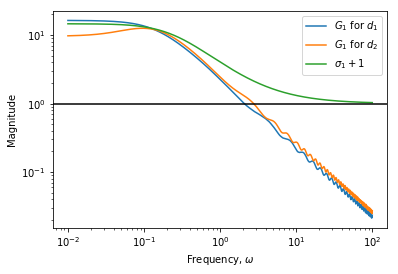
\includegraphics[width=\linewidth]{Figures/InputSaturation1}
 		\captionof{figure}{Graphical representation of criteria outlined in Equation~\ref{eq:Input saturation of disturbances}, for $e_1$}
 		\label{fig:Input Saturation 1}
 	\end{minipage}%
 	\hfill
 	\begin{minipage}{.48\textwidth}
 		\centering
 		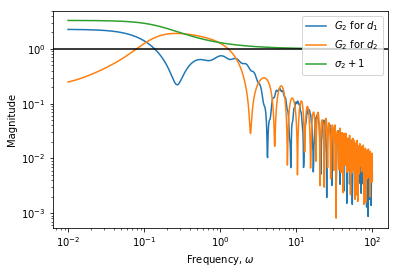
\includegraphics[width=\linewidth]{Figures/InputSaturation2}
 		\captionof{figure}{Graphical representation of criteria outlined in Equation~\ref{eq:Input saturation of disturbances}, for $e_2$}
 		\label{fig:Input Saturation 2}
 	\end{minipage}
 \end{figure}

 \begin{figure}[H]
	\centering
	\begin{minipage}{.48\textwidth}
		\centering
		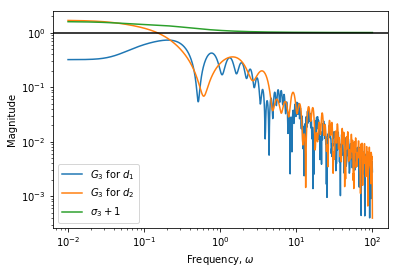
\includegraphics[width=\linewidth]{Figures/InputSaturation3}
		\captionof{figure}{Graphical representation of criteria outlined in Equation~\ref{eq:Input saturation of disturbances}, for $e_3$}
		\label{fig:Input Saturation 3}
	\end{minipage}%
	\hfill
	\begin{minipage}{.48\textwidth}
		\centering
		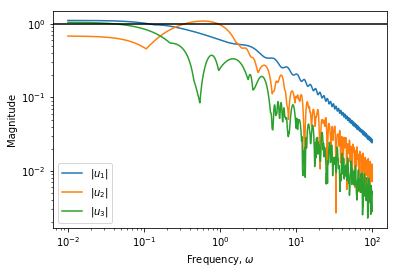
\includegraphics[width=\linewidth]{Figures/Input_Requirements}
		\captionof{figure}{The required controller input values for the worst case }
		\label{fig:Input Requirements}
	\end{minipage}
\end{figure}

When considering Figure~\ref{fig:Input Saturation 1}, it is clear that the input into the controller (controlling $y_1$) is saturated at low frequencies. This is due to the effects that $d_1$ has on the system. It is clear that a maximum change in the feed flow rate, will result in the reflux flow rate flow being saturated. This translates to a fully open or fully closed control valve in this section of the plant. There are two solutions to the problem, namely

\begin{enumerate}
	\item Install a bigger control valve (and therefore line size) on the reflux stream. This change will impact the mathematical model by changing the gain and response times in the first row of transfer function matrix $G(s)$. This speed up the dynamics of the system, and result in higher minimum singular values for $S(s)$, especially at low frequencies where the problem is experienced. Better disturbance rejection will result.
	
	\item Lower the maximum designed for disturbance size. This can be done by tighter control upstream from the distillation column (by the flow regulator/controller indicated in Figure~\ref{fig:PFD}).
	
\end{enumerate}   

Both actions will take considerable time to implement, as the effect of tighter flow control will effect the reactor vessel's control as well. A bigger, or more sophisticated control valve, will have a installation cost, as well as a downtime, as well as recommissioning of the system, production cost implication. 

From Figure~\ref{fig:Input Saturation 2} it is clear that acceptable control is possible, since the second input to the controller is saturated by neither disturbance changes (for all frequencies).

Regarding Figure~\ref{fig:Input Saturation 3}, it is clear that disturbance rejection is again not acceptable, as the third input to the controller ($e_3$) is saturated when disturbance $d_2$ is at it's maximum feed value. When relating back to the physical process, this means that the stream pressure control valve, fully closes when the feed temperature rises to 106 $^{\circ}$F or fully opens when the feed temperature drops to 58 $^{\circ}$F. To solve this problem there again exists a few solutions, namely

\begin{enumerate}
	\item Increase the size of the control valve. When doing this, it is imperative that the compressors in the stream line's design also be reviewed, as it may be required that a higher stream flow rate be required at the lowest disturbance value. The major downside of this option, is that there is no compensation for when the feed temperature rises to the maximum disturbance value. Even the bigger control valve will still fully close.
	\item Decrease the disturbance limit values. This is again the most straightforward method to increase the effectiveness of disturbance rejection over the distillation column. This can be done by implementing tighter control over the feed heat exchanger unit (indicated in Figure~\ref{fig:PFD}). Methods to implement tighter control will be to increase the controller gain of the unit (an decreasing the amount of integral control). Implementing a feed forward controller on the heat exchanger unit by adding the working fluid's temperature as measured variable is another option (although this will not be the most cost effective solution).
	\item Change the controlled variable $y_3$. By changing the controlled variable $y_3$ from the temperature on tray \#19, to the boil-up ratio will reduce the response time in dynamics of the third row in $G(s)$. This will lead to higher singular values in $S(s)$, especially at low frequencies, and disturbance rejection performance criteria will be met. This solution has the downside that the bottoms composition will not be controlled directly. Since the production is more interested in the quality of the distillate composition (as this is where the ethanol product is), this is not a major loss and the solution can be considered. A full controllability analysis will have to be conducted on the new system if this is the chosen solution, as the dynamics of the whole MIMO transfer function model will change.
\end{enumerate}

Figure~\ref{fig:Input Requirements} illustrates the required input variables ($u_i$) for maximum disturbance rejection. The figure reiterates the problems experienced in Figure~\ref{fig:Input Saturation 1} and Figure~\ref{fig:Input Saturation 3}, where the inputs required for disturbance rejection will saturate the controller.  


\newpage

\section{Changing the System Bounds}
\subsection{Disturbance Rejection and Input Saturation}

This section will look at the proposed changes stated in Section~\ref{sec:Analysis for acceptable control:disturbances}. Since there is no information on the current controllers and final control elements employed on site, investigation into changes of the control hardware will not be conducted. This is purely due to

\begin{enumerate}
	\item Lack of information about current control infrastructure. 
	\item Lack of a first principles mathematical model, or Aspen simulation where the sizes of the control elements can be changed at will without any additional cost.
\end{enumerate}

The proposed changes to the perimeters of the control system will therefore be investigated. As mentioned in Section~\ref{sec:Analysis for acceptable control:disturbances}, disturbance rejection is required for a too high range of both disturbances. In order to rectify the situation, the ranges where adjusted. This in turn caused the scaled system to change, and new responses resulted. Table~\ref{tab:Disturbance_variables_updated_scaling} contains more information with regard to the proposed ranges.

\begin{table}[H]
	\centering
	\caption{The new proposed boundaries of the disturbance variables in the system.}
	\begin{tabular}{cccc}
		\hline
		\textbf{\begin{tabular}[c]{@{}c@{}}Disturbance\\   Variable\end{tabular}} & \textbf{\begin{tabular}[c]{@{}c@{}}Lower \\ Constraint\end{tabular}} & \textbf{\begin{tabular}[c]{@{}c@{}}Upper \\ Constraint\end{tabular}} & \textbf{\begin{tabular}[c]{@{}c@{}}Steady State \\ Value\end{tabular}} \\\hline
		d1, Feed Flow Rate            & 0.65                       & 1.0                       & 0.8                         \\
		d2, Feed Temperature          & 60                        & 95                       & 78                         
		\\\hline      
	\end{tabular}
	\label{tab:Disturbance_variables_updated_scaling}
\end{table}

This led to a new scaling matrix

\begin{equation}
	D_d = \begin{bmatrix}
	0.2 & 0 \\
	0 & 18\\
	\end{bmatrix}
\end{equation}

and a new disturbance matrix

\begin{equation}
G_d(s) = \begin{bmatrix}
G_{d11} & G_{d12} \\
G_{d21} & G_{d22} \\
G_{d31} & G_{d32} \\
\end{bmatrix} = \begin{bmatrix}
\frac{2.8e^{-12s}}{6.2s+1} & \frac{-1800(0.028952s+0.0011)e^{-2.66s}}{(7.85s+1)(4.63s+1)} \\
\frac{10.6e^{-10.5s}}{6.9s+1} & \frac{-1800(-0.062784s+0.0032)e^{-3.44s}}{(7.29s+1)(8.94s+1)} \\
\frac{-0.577e^{-0.6s}}{7.01s+1} & \frac{1.44e^{-2.6s}}{7.76s+1}
\end{bmatrix}
\end{equation}

The same mathematical procedure is then followed as outlined in Section~\ref{sec:Analysis for acceptable control:disturbances}, to establish whether acceptable disturbance rejection can take place. The following figures result.

\begin{figure}[H]
	\centering
	\includegraphics[width=0.7\linewidth]{"Figures/Disturbance Analysis 2 Max Norm_Updated"}
	\caption{The effect of disturbances on input saturation.}
	\label{fig:disturbance-analysis-2-max-norm_updated}
\end{figure}

 \begin{figure}[H]
	\centering
	\begin{minipage}{.48\textwidth}
		\centering
		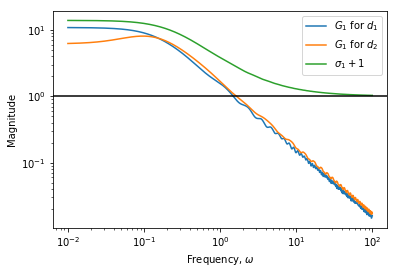
\includegraphics[width=\linewidth]{Figures/InputSaturation1_Updated}
		\captionof{figure}{Graphical representation of criteria outlined in Equation~\ref{eq:Input saturation of disturbances}, for $e_1$}
		\label{fig:Input Saturation 1_Updated}
	\end{minipage}%
	\hfill
	\begin{minipage}{.48\textwidth}
		\centering
		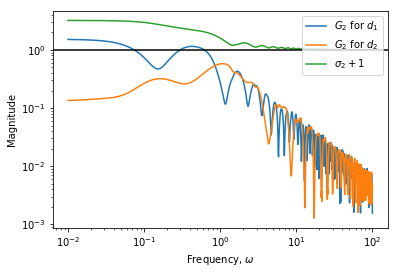
\includegraphics[width=\linewidth]{Figures/InputSaturation2_Updated}
		\captionof{figure}{Graphical representation of criteria outlined in Equation~\ref{eq:Input saturation of disturbances}, for $e_2$}
		\label{fig:Input Saturation 2_Updated}
	\end{minipage}
\end{figure}

\begin{figure}[H]
	\centering
	\begin{minipage}{.48\textwidth}
		\centering
		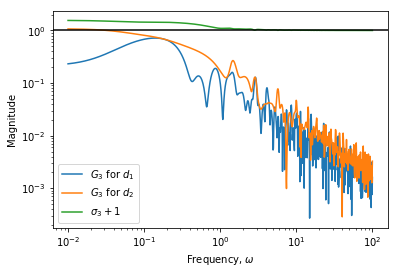
\includegraphics[width=\linewidth]{Figures/InputSaturation3_Updated}
		\captionof{figure}{Graphical representation of criteria outlined in Equation~\ref{eq:Input saturation of disturbances}, for $e_3$}
		\label{fig:Input Saturation 3_Updated}
	\end{minipage}%
	\hfill
	\begin{minipage}{.48\textwidth}
		\centering
		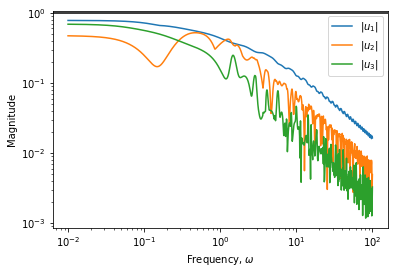
\includegraphics[width=\linewidth]{Figures/Input_Requirements_Updated}
		\captionof{figure}{The required controller input values for the worst case }
		\label{fig:Input Requirements_Updated}
	\end{minipage}
\end{figure}
\newpage

\section{Uncertainty and Robustness}

In this section the uncertainty model will be derived to include various aspects where uncertainly is present.

Looking at the method in which the model is derived, the main uncertainties in this description of the process are

\begin{enumerate}
	\item  Parametric uncertainty. This is from the fact that the model is fitted. The variables used for fitting the models were rounded to produce numbers that are easy to work with. This causes uncertainty regarding the accuracy of the model, as all the variables may be wrong by a fractional amount.
	\item Uncertainty due to neglected dynamics. This will most certainly be included in the current model, as the core principle behind fitting dynamic models to experimental data involves the simplification of multi order differential equations to first or second order systems. 
\end{enumerate}

The above list contains the uncertainties that are certain. Some uncertainties are unlikely. These uncertainties will not be considered when deriving the uncertainty model. This includes

\begin{enumerate}
	\item Neglected delays. This can be excluded, as all the modelled equations contains delays. The uncertainty regarding the delays will therefore only be analysed when looking at the parametric uncertainty of the values of $\theta_{ij}$.
\end{enumerate}

\subsection{Choosing the Uncertainty Weight Form}

A major thing to consider when setting up the uncertainty model is which uncertainty weight form to use. The two major weights to choose from are

\begin{enumerate}
	\item Additive uncertainty.
	\item Multiplicative weight uncertainty.
\end{enumerate}

The major deciding factor for the choice will be the ease of fitting the uncertainty weight to the smallest uncertainty radius of all possible plants ($\Pi$). In mathematical terms the radius can be described as 
\begin{equation}
	l_A = \max_{G_p \epsilon \Pi} |G_p(j\omega) - G(j\omega)|
\end{equation}

for additive uncertainty, and 

\begin{equation}
	l_I = \max_{G_p \epsilon \Pi} |\frac{G_p(j\omega) - G(j\omega)}{G(j\omega)}|
\end{equation}

for multiplicative uncertainty. In the above equations $G_p(j\omega)$ refers to the perturbed model. The complete uncertainty analysis was pulled from \textcite{skogestad}, and for more information regarding the concepts please consult the reference material. Preferably the uncertainty weight should have the lowest possible order. The relative shape difference between the two uncertainty descriptions are displayed in Figure~\ref{fig:uncertaintyadditivevsmultiplicative}.

\begin{figure}[H]
	\centering
	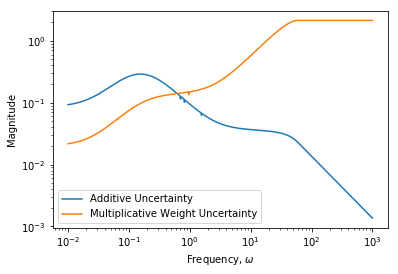
\includegraphics[width=0.7\linewidth]{Figures/Uncertainty_Additive_vs_Multiplicative}
	\caption{A comparison between additive and multiplicative uncertainty weight requirements, when analysing parametric uncertainty of a first order plus dead time equation.}
	\label{fig:uncertaintyadditivevsmultiplicative}
\end{figure}

From the picture it is clear that drastically different shapes for $l_A$ and $l_I$ is obtained using the uncertainty descriptions. When the two are compared, it is clear that

\begin{enumerate}
	\item The additive uncertainty will require at least one lead and two lag term to get an acceptable fit. Only using one lag will lead to an over estimated uncertainty for low frequencies. To gain an even tighter fit one additional lag and lead term can be added. This however will result in a very complex uncertainty weight.
	\item The multiplicative uncertainty requires only one lag and one lead to get an acceptable fit. For a tighter fit, one additional lag and lead can be added. This is not entirely necessary, as the frequencies where uncertainty is over estimated are in the crossover frequency range. This is therefore a very conventional fit. In later sections the benefit of this estimation with regard to unmodelled dynamics uncertainty is discussed. 
\end{enumerate}

For this uncertainty description multiplicative weights will be used to describe the uncertainty. This is simply due to the ease of fitting the multiplicative weights to the uncertainty descriptions.

\subsection{Parametric Uncertainty}

As mentioned in the previous section, parametric uncertainty is inherent to the model. Using the data and subsequent models fit to the data, is was decided to

\begin{itemize}
	\item Estimate the uncertainty of all gains as 2 \%.
	\item Estimate the uncertainty of all time constants as 10 \%.
	\item Estimate the uncertainty of all time delays as 2 \%.
\end{itemize}

The values above are chosen based on the distribution of data points in key places, during the step test analysis. The steady state gains were relatively clear due to a small variance distribution of particles along the horizontal lines (steady state) in the time domain responses. The same principle applies to the time it takes before a response is observed. The critical point is quite easily identifiable, and the first order plus dead time models can capture the dead time in the system with little uncertainty regarding the value of the dead time. This is most definitely due to high quality measuring devices that can deliver consistent accurate measured values.

It is only in the middle of the step responses that a deviation in measured value occurred. This is captured in a lower local $R^2$ value in this region of the step response. This is the reason why the time constants are more uncertain than the other parameters.

All the first order plus dead time transfer functions within $G(s)$ have the relatively the same shape (their uncertainty descriptions are the same). For this reason, the same fitting function was used to describe the performance weights. This function is

\begin{equation}
	\label{eq:Uncertainty weights}
	w_{Ii} = \frac{Ts + k_1}{(T/2.5)s + 1}
\end{equation}

This is the minimum order uncertainty weight that could be fit to the functions, and was chosen to simplify the uncertainty model. Table~\ref{tab:Uncertainty description G(s)} contains all the various constants for the uncertainty model of $G(s)$.

\begin{table}[H]
	\centering
	\begin{tabular}{cccc}
		\hline
		\textbf{Transfer Function} & \textbf{Uncertainty Weight} & \textbf{$T$} & \textbf{$k_1$} \\
		\hline
		$G_{11}$                        & $w_{I11}$                  & 0.7        & 0.02        \\
		$G_{12}$                        & $w_{I12}$                  & 0.5        & 0.015       \\
		$G_{13}$                        & $w_{I13}$                  & 0.55       & 0.04        \\
		$G_{21}$                        & $w_{I21}$                  & 0.3        & 0.06        \\
		$G_{22}$                        & $w_{I22}$                  & 0.2        & 0.05        \\
		$G_{23}$                        & $w_{I23}$                  & 0.75       & 0.035       \\
		$G_{31}$                        & $w_{I31}$                  & 0.07       & 0.09        \\
		$G_{32}$                        & $w_{I32}$                  & 0.05       & 0.1       \\\hline 
	\end{tabular}
	\caption{The uncertainty model of the first order plus dead time components of $G(s)$}
	\label{tab:Uncertainty description G(s)}
\end{table}

Figure~\ref{fig:Uncertainty wI 11} and Figure~\ref{fig:Uncertainty wI 13} graphically illustrates the procedure of fitting the uncertainty curves. The complete set of fitted figures can be found in the Appendix.

\begin{figure}[H]
	\centering
	\begin{minipage}{.48\textwidth}
		\centering
		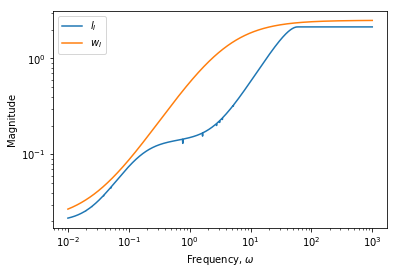
\includegraphics[width=\linewidth]{Figures/Uncertainty_wI_11}
		\captionof{figure}{The uncertainty weight of transfer function $G_{11}$.}
		\label{fig:Uncertainty wI 11}
	\end{minipage}%
	\hfill
	\begin{minipage}{.48\textwidth}
		\centering
		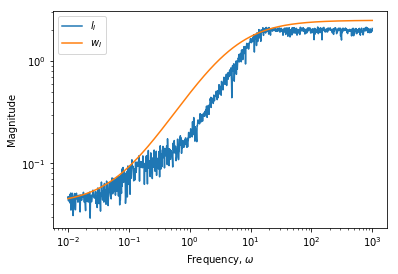
\includegraphics[width=\linewidth]{Figures/Uncertainty_wI_13}
		\captionof{figure}{The uncertainty weight of transfer function $G_{13}$.}
		\label{fig:Uncertainty wI 13}
	\end{minipage}
\end{figure}

From Figure~\ref{fig:Uncertainty wI 13} it is apparent that the optimization function used to solve the "worst case" combination of the parameters did not return a smooth solution. Increasing the number of start for the optimization function had no effect. In fact, al the functions with negative gain did not return a smooth curve when passed to the optimization function. Unfortunately, due to time constraints, the matter could not be investigated any further. The performance weight was just adjusted to lie on the top part of the fluctuating curve.

The transfer function $G_{33}$, required special attention, as this was not simply a first order plus dead time model. There are more time constants (a total number of three) in the function. All variables carried the same uncertainty as specified above. The ultimate performance weight function was determined as

\begin{equation}
	w_{I33} = \frac{(0.8s + 8)(0.55s + 0.0095)}{(11s + 1)(0.015s + 1)}
\end{equation}

The fitting of the uncertainty weight to $l_I$ is displayed in Figure~\ref{fig:uncertaintywi33}.

\begin{figure}[H]
	\centering
	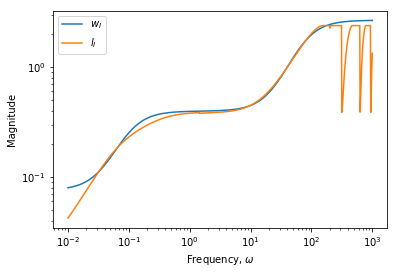
\includegraphics[width=0.7\linewidth]{Figures/Uncertainty_wI_33}
	\caption{The uncertainty weight of transfer function $G_{33}$.}
	\label{fig:uncertaintywi33}
\end{figure}

A much tighter uncertainty weight fit was achieved using this model. The weight described in Equation~\ref{eq:Uncertainty weights} was too inaccurate. Big over estimates would have been made at very low frequencies, as well as at crossover frequencies.

The same procedure was carried out to construct an uncertainty model for $G_d(s)$. There were again a lot of first order plus dead time elements in the system. Equation~\ref{eq:Uncertainty weights} was used to fit all of the multiplicative uncertainty descriptions. Table contains the resulting calculated constants.

\begin{table}[H]
	\centering
	\begin{tabular}{cccc}
		\hline
		\textbf{Transfer Function} & \textbf{Uncertainty Weight} & \textbf{$T$} & \textbf{$k_1$} \\
		\hline
		$G_{d11}$                        & $w_{Id11}$                  & 1.5        & 0.01        \\
		$G_{d21}$                        & $w_{Id21}$                  & 0.8        & 0.015        \\
		$G_{d31}$                        & $w_{Id31}$                  & 0.8       & 0.015        \\
		$G_{d32}$                        & $w_{Id 32}$                 & 0.8       & 0.015       \\\hline 
	\end{tabular}
	\caption{The uncertainty model of the first order plus dead time components of $G_d(s)$}
	\label{tab:Uncertainty description Gd(s)}
\end{table}

In $G_d(s)$ there are also two transfer function equation that are more complicated. The multiplicative uncertainty form has a shape that will require two lags and two leads in an uncertainty weight. The additive uncertainty form however only requires two lags and one lead. The uncertainty form slected for these two elements was therefore the additive form. The uncertainty weights calculated are

\begin{equation}
	w_{A12} = \frac{6.94(-0.3s+1)}{(s+1)^2}
\end{equation}

and 

\begin{equation}
w_{A22} = \frac{11(35s+1)}{(9.65s+1)^2}
\end{equation}

Figure~\ref{fig:Uncertainty wI Gd12} and Figure~\ref{fig:Uncertainty wI Gd22} displays the uncertainty weights fit for the above two equations.

\begin{figure}[H]
	\centering
	\begin{minipage}{.48\textwidth}
		\centering
		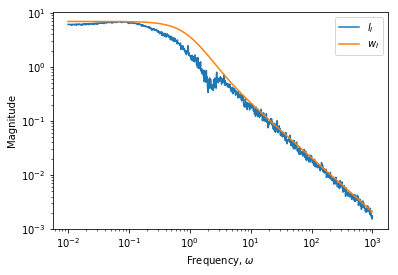
\includegraphics[width=\linewidth]{Figures/Uncertainty_wI_Gd12}
		\captionof{figure}{The uncertainty weight of transfer function $Gd_{12}$.}
		\label{fig:Uncertainty wI Gd12}
	\end{minipage}%
	\hfill
	\begin{minipage}{.48\textwidth}
		\centering
		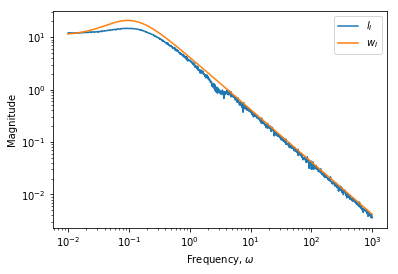
\includegraphics[width=\linewidth]{Figures/Uncertainty_wI_Gd22}
		\captionof{figure}{The uncertainty weight of transfer function $Gd_{22}$.}
		\label{fig:Uncertainty wI Gd22}
	\end{minipage}
\end{figure}
\newpage

\section{Performance Measurement}
\label{sec:Performance Measurement}
In order to adequately test the performance the system (nominal and robust performance), and acceptable and relative performance weight has to be formulated. This section entails the development of just such a function. 

One major consideration in the performance weights are the disturbance dynamics. When designing a controller that has to reject disturbances up to an acceptable degree, the performance weight ($w_P$)can be chosen to closely represent $G_d$ in SISO systems. Dosing this for MIMO is slightly harder, as the directions of the various disturbances play a major role in the disturbance rejection dynamics. Simply taking the singular value of $G_d$ does not represent the disturbance inputs adequately.

Rejecting the disturbances, however, is not the only consideration. The performance of set-point tracking dynamics also has to be taken into account. A major role player in analysing this is the bandwidth limits calculated for all of the different inputs (see Section~\ref{sec:Bandwidths}). A common choice for the form of the performance weight is 

\begin{equation}
	W_P = \textrm{diag}\{w_{Pi}\}
\end{equation}

where

\begin{equation}
	\label{eq:Performance Weigths}
	w_{Pi} = \frac{s/M_i + \omega^*_{Bi}}{s + \omega^*_{Bi}A_i} , A_i < 1
\end{equation}

Using Equation~\ref{eq:Performance Weigths}, and selecting a small value for $A_i$ ensures approximate integral action when analysing the weighted sensitivity at very low frequencies ($\omega = 0$). $M_i$ is mostly selected as 2. This value limits the required performance at high frequencies, and at the crossover frequencies, where $\sigma(S(j\omega))>1$. For this preliminary performance weight analysis, the value for $M_i$ was chosen to be a constant 2. The bandwidths were chosen as the bandwidth limits outlined in Section~\ref{sec:Bandwidths}. The value of $A_i$ was chosen so that $A_i - \sigma_i(S(j10^{-2})) = 0$. Using this equation will ensure very tight performance requirements between the frequencies $\omega = 10^{-2}$ and $\omega^*_{Bi}$, for all of the output variables. 

The proposed performance weight equation is

\begin{equation}
	W_P = \begin{bmatrix}
	\frac{s/2 + 0.46}{s+ 0.46(0.079)} & 0 & 0\\
	0 & \frac{s/2 + 0.46}{s+ 0.46(0.395)} & 0\\
	0 & 0 & \frac{s/2 + 1}{s+ 1(0.692)}
	\end{bmatrix}
\end{equation}
\newpage

\section{Conclusions}

Following the controllability analysis performed it can be stated that

\begin{enumerate}
	\item The process contains good controllability characteristics. The bandwidth limitations on the process are reasonable, and will allow for the implementation of a controller.
	\item The bounds set on disturbance variation were too ambitious, and the process may not be able to reject disturbances with magnitude close to the upper or lower bounds.
	\item The bounds set on maximum set-point variation also appeared to be too ambitious. Especially the maximum set-point variation of 8~$\celsius$ on the bottom tray temperature will not be realizable in the system.
	\item The unstable nodes in the MIMO system were calculated and analysed successfully.
	\item An acceptable uncertainty model was constructed to describe the various uncertainties within the model.
	\item A performance weight was constructed to measure the nominal and robust performance of the process once the controller design has begun.
\end{enumerate}

Recommendations and processes that will have to follow are

\begin{enumerate}
	\item The controller for the process will have to be designed, using various methods (decentralized, $H^\infty$-design).
	\item When a controller transfer function has been designed, the nominal and robust stability and performance of the process has to be verified.
	\item After the analysis and design, the implementation of the controller can commence.
\end{enumerate}

\newpage
\printbibliography
\appendix
\newpage

\section{Appendix}

The figures below contain all the fitting curves used to obtain the uncertainty weights.

\begin{figure}[H]
	\centering
	\begin{minipage}{.48\textwidth}
		\centering
		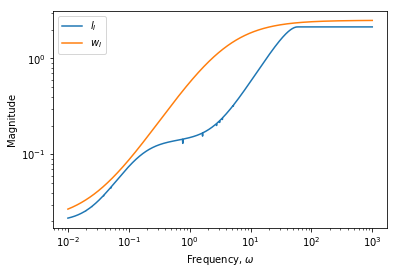
\includegraphics[width=\linewidth]{Figures/Uncertainty_wI_11}
		\captionof{figure}{The uncertainty weight of transfer function $G_{11}$.}
	\end{minipage}%
	\hfill
	\begin{minipage}{.48\textwidth}
		\centering
		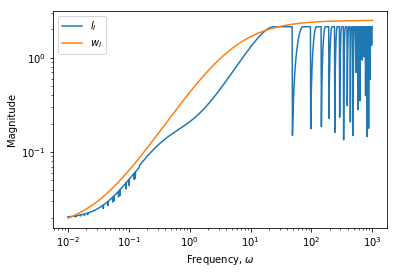
\includegraphics[width=\linewidth]{Figures/Uncertainty_wI_12}
		\captionof{figure}{The uncertainty weight of transfer function $G_{12}$.}
	\end{minipage}
\end{figure}

\begin{figure}[H]
	\centering
	\begin{minipage}{.48\textwidth}
		\centering
		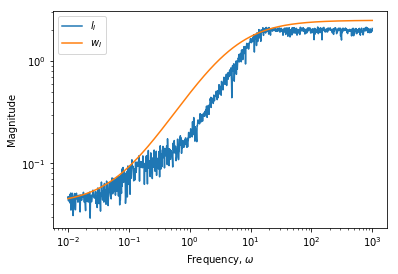
\includegraphics[width=\linewidth]{Figures/Uncertainty_wI_13}
		\captionof{figure}{The uncertainty weight of transfer function $G_{13}$.}
	\end{minipage}%
	\hfill
	\begin{minipage}{.48\textwidth}
		\centering
		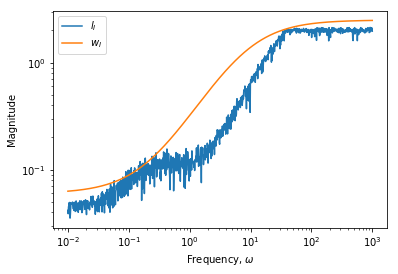
\includegraphics[width=\linewidth]{Figures/Uncertainty_wI_21}
		\captionof{figure}{The uncertainty weight of transfer function $G_{21}$.}
	\end{minipage}
\end{figure}

\begin{figure}[H]
	\centering
	\begin{minipage}{.48\textwidth}
		\centering
		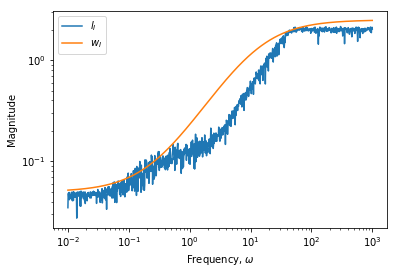
\includegraphics[width=\linewidth]{Figures/Uncertainty_wI_22}
		\captionof{figure}{The uncertainty weight of transfer function $G_{22}$.}
	\end{minipage}%
	\hfill
	\begin{minipage}{.48\textwidth}
		\centering
		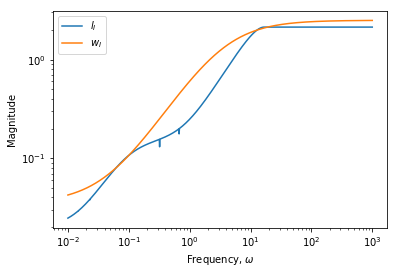
\includegraphics[width=\linewidth]{Figures/Uncertainty_wI_23}
		\captionof{figure}{The uncertainty weight of transfer function $G_{23}$.}
	\end{minipage}
\end{figure}

\begin{figure}[H]
	\centering
	\begin{minipage}{.48\textwidth}
		\centering
		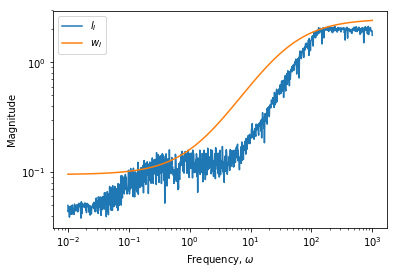
\includegraphics[width=\linewidth]{Figures/Uncertainty_wI_31}
		\captionof{figure}{The uncertainty weight of transfer function $G_{31}$.}
	\end{minipage}%
	\hfill
	\begin{minipage}{.48\textwidth}
		\centering
		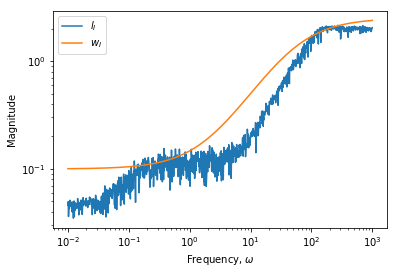
\includegraphics[width=\linewidth]{Figures/Uncertainty_wI_32}
		\captionof{figure}{The uncertainty weight of transfer function $G_{32}$.}
	\end{minipage}
\end{figure}

\begin{figure}[H]
	\centering
	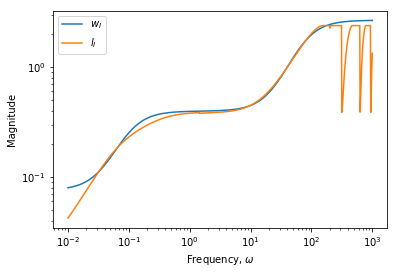
\includegraphics[width=.8\linewidth]{Figures/Uncertainty_wI_33}
	\captionof{figure}{The uncertainty weight of transfer function $G_{33}$.}
\end{figure}
\renewcommand{\thefigure}{\thesection.\arabic{figure}}
\renewcommand{\thetable}{\thesection.\arabic{table}}
\renewcommand{\thepage}{\thesection.\arabic{page}}
\end{document}